% Options for packages loaded elsewhere
\PassOptionsToPackage{unicode}{hyperref}
\PassOptionsToPackage{hyphens}{url}
%
\documentclass[
]{book}
\usepackage{amsmath,amssymb}
\usepackage{iftex}
\ifPDFTeX
  \usepackage[T1]{fontenc}
  \usepackage[utf8]{inputenc}
  \usepackage{textcomp} % provide euro and other symbols
\else % if luatex or xetex
  \usepackage{unicode-math} % this also loads fontspec
  \defaultfontfeatures{Scale=MatchLowercase}
  \defaultfontfeatures[\rmfamily]{Ligatures=TeX,Scale=1}
\fi
\usepackage{lmodern}
\ifPDFTeX\else
  % xetex/luatex font selection
\fi
% Use upquote if available, for straight quotes in verbatim environments
\IfFileExists{upquote.sty}{\usepackage{upquote}}{}
\IfFileExists{microtype.sty}{% use microtype if available
  \usepackage[]{microtype}
  \UseMicrotypeSet[protrusion]{basicmath} % disable protrusion for tt fonts
}{}
\makeatletter
\@ifundefined{KOMAClassName}{% if non-KOMA class
  \IfFileExists{parskip.sty}{%
    \usepackage{parskip}
  }{% else
    \setlength{\parindent}{0pt}
    \setlength{\parskip}{6pt plus 2pt minus 1pt}}
}{% if KOMA class
  \KOMAoptions{parskip=half}}
\makeatother
\usepackage{xcolor}
\usepackage{color}
\usepackage{fancyvrb}
\newcommand{\VerbBar}{|}
\newcommand{\VERB}{\Verb[commandchars=\\\{\}]}
\DefineVerbatimEnvironment{Highlighting}{Verbatim}{commandchars=\\\{\}}
% Add ',fontsize=\small' for more characters per line
\usepackage{framed}
\definecolor{shadecolor}{RGB}{248,248,248}
\newenvironment{Shaded}{\begin{snugshade}}{\end{snugshade}}
\newcommand{\AlertTok}[1]{\textcolor[rgb]{0.94,0.16,0.16}{#1}}
\newcommand{\AnnotationTok}[1]{\textcolor[rgb]{0.56,0.35,0.01}{\textbf{\textit{#1}}}}
\newcommand{\AttributeTok}[1]{\textcolor[rgb]{0.13,0.29,0.53}{#1}}
\newcommand{\BaseNTok}[1]{\textcolor[rgb]{0.00,0.00,0.81}{#1}}
\newcommand{\BuiltInTok}[1]{#1}
\newcommand{\CharTok}[1]{\textcolor[rgb]{0.31,0.60,0.02}{#1}}
\newcommand{\CommentTok}[1]{\textcolor[rgb]{0.56,0.35,0.01}{\textit{#1}}}
\newcommand{\CommentVarTok}[1]{\textcolor[rgb]{0.56,0.35,0.01}{\textbf{\textit{#1}}}}
\newcommand{\ConstantTok}[1]{\textcolor[rgb]{0.56,0.35,0.01}{#1}}
\newcommand{\ControlFlowTok}[1]{\textcolor[rgb]{0.13,0.29,0.53}{\textbf{#1}}}
\newcommand{\DataTypeTok}[1]{\textcolor[rgb]{0.13,0.29,0.53}{#1}}
\newcommand{\DecValTok}[1]{\textcolor[rgb]{0.00,0.00,0.81}{#1}}
\newcommand{\DocumentationTok}[1]{\textcolor[rgb]{0.56,0.35,0.01}{\textbf{\textit{#1}}}}
\newcommand{\ErrorTok}[1]{\textcolor[rgb]{0.64,0.00,0.00}{\textbf{#1}}}
\newcommand{\ExtensionTok}[1]{#1}
\newcommand{\FloatTok}[1]{\textcolor[rgb]{0.00,0.00,0.81}{#1}}
\newcommand{\FunctionTok}[1]{\textcolor[rgb]{0.13,0.29,0.53}{\textbf{#1}}}
\newcommand{\ImportTok}[1]{#1}
\newcommand{\InformationTok}[1]{\textcolor[rgb]{0.56,0.35,0.01}{\textbf{\textit{#1}}}}
\newcommand{\KeywordTok}[1]{\textcolor[rgb]{0.13,0.29,0.53}{\textbf{#1}}}
\newcommand{\NormalTok}[1]{#1}
\newcommand{\OperatorTok}[1]{\textcolor[rgb]{0.81,0.36,0.00}{\textbf{#1}}}
\newcommand{\OtherTok}[1]{\textcolor[rgb]{0.56,0.35,0.01}{#1}}
\newcommand{\PreprocessorTok}[1]{\textcolor[rgb]{0.56,0.35,0.01}{\textit{#1}}}
\newcommand{\RegionMarkerTok}[1]{#1}
\newcommand{\SpecialCharTok}[1]{\textcolor[rgb]{0.81,0.36,0.00}{\textbf{#1}}}
\newcommand{\SpecialStringTok}[1]{\textcolor[rgb]{0.31,0.60,0.02}{#1}}
\newcommand{\StringTok}[1]{\textcolor[rgb]{0.31,0.60,0.02}{#1}}
\newcommand{\VariableTok}[1]{\textcolor[rgb]{0.00,0.00,0.00}{#1}}
\newcommand{\VerbatimStringTok}[1]{\textcolor[rgb]{0.31,0.60,0.02}{#1}}
\newcommand{\WarningTok}[1]{\textcolor[rgb]{0.56,0.35,0.01}{\textbf{\textit{#1}}}}
\usepackage{longtable,booktabs,array}
\usepackage{calc} % for calculating minipage widths
% Correct order of tables after \paragraph or \subparagraph
\usepackage{etoolbox}
\makeatletter
\patchcmd\longtable{\par}{\if@noskipsec\mbox{}\fi\par}{}{}
\makeatother
% Allow footnotes in longtable head/foot
\IfFileExists{footnotehyper.sty}{\usepackage{footnotehyper}}{\usepackage{footnote}}
\makesavenoteenv{longtable}
\usepackage{graphicx}
\makeatletter
\def\maxwidth{\ifdim\Gin@nat@width>\linewidth\linewidth\else\Gin@nat@width\fi}
\def\maxheight{\ifdim\Gin@nat@height>\textheight\textheight\else\Gin@nat@height\fi}
\makeatother
% Scale images if necessary, so that they will not overflow the page
% margins by default, and it is still possible to overwrite the defaults
% using explicit options in \includegraphics[width, height, ...]{}
\setkeys{Gin}{width=\maxwidth,height=\maxheight,keepaspectratio}
% Set default figure placement to htbp
\makeatletter
\def\fps@figure{htbp}
\makeatother
\setlength{\emergencystretch}{3em} % prevent overfull lines
\providecommand{\tightlist}{%
  \setlength{\itemsep}{0pt}\setlength{\parskip}{0pt}}
\setcounter{secnumdepth}{5}
\usepackage{booktabs}
\ifLuaTeX
  \usepackage{selnolig}  % disable illegal ligatures
\fi
\usepackage[]{natbib}
\bibliographystyle{plainnat}
\usepackage{bookmark}
\IfFileExists{xurl.sty}{\usepackage{xurl}}{} % add URL line breaks if available
\urlstyle{same}
\hypersetup{
  pdftitle={Introduction to R 2024},
  hidelinks,
  pdfcreator={LaTeX via pandoc}}

\title{Introduction to R 2024}
\author{}
\date{\vspace{-2.5em}June 11 - June 12 2024}

\usepackage{amsthm}
\newtheorem{theorem}{Theorem}[chapter]
\newtheorem{lemma}{Lemma}[chapter]
\newtheorem{corollary}{Corollary}[chapter]
\newtheorem{proposition}{Proposition}[chapter]
\newtheorem{conjecture}{Conjecture}[chapter]
\theoremstyle{definition}
\newtheorem{definition}{Definition}[chapter]
\theoremstyle{definition}
\newtheorem{example}{Example}[chapter]
\theoremstyle{definition}
\newtheorem{exercise}{Exercise}[chapter]
\theoremstyle{definition}
\newtheorem{hypothesis}{Hypothesis}[chapter]
\theoremstyle{remark}
\newtheorem*{remark}{Remark}
\newtheorem*{solution}{Solution}
\begin{document}
\maketitle

{
\setcounter{tocdepth}{1}
\tableofcontents
}
\chapter{Introduction}\label{introduction}

Welcome to CBW's Introduction to R 2024 Workshop!

Before continuing, ensure to register, complete your pre-work (below) and ensure your zoom is functional.

\section{Pre-Workshop Materials}\label{prework}

Click \href{https://forms.gle/xba2wVbLXtC1E1Dx9}{here} for the pre-work. This includes programs to install.

\section*{Meet Your Faculty}\label{nice-label}
\addcontentsline{toc}{section}{Meet Your Faculty}

Here's the team!

\subsection*{\texorpdfstring{Frances Wong (she/her) }{Frances Wong  (she/her) }}\label{frances-wong-sheher}
\addcontentsline{toc}{subsection}{Frances Wong (she/her) }

\begin{center}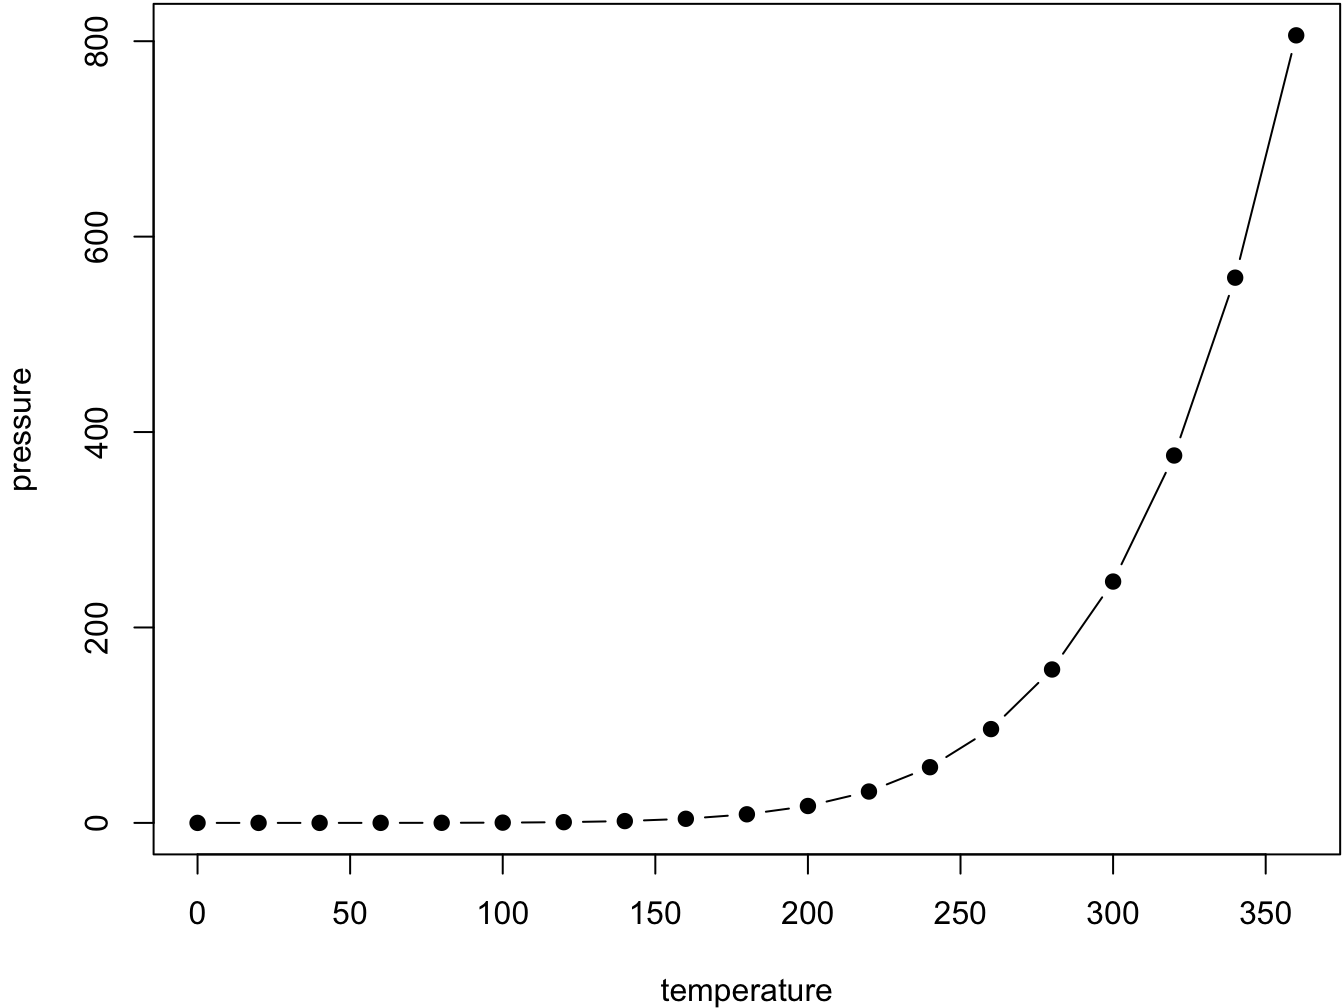
\includegraphics[width=0.65\linewidth]{./_main_files/figure-html/nice-fig-1} \end{center}

\begin{quote}
Assistant Professor, Teaching Stream,
University of Toronto Missisauga

--- \href{mailto:frances.wong@utoronto.ca}{\nolinkurl{frances.wong@utoronto.ca}}
\end{quote}

Frances Wong is an assistant professor, teaching stream, at the University of Toronto
Mississauga Department of Biology. She is interested in how dynamic cell populations make
decisions (sometimes incorrectly!) during development. Frances used a systems biology
approach to investigate human placenta development by isolating single cells at multiple time
points during early development to computationally assemble a cell atlas of first trimester
development. Currently, Frances incorporates computational literacy as a core course
objective in biology courses she teaches to empower over 1000 students to analyze the data
they collect each semester.

\subsection*{\texorpdfstring{Andrés Melani (he/him) }{Andrés Melani  (he/him) }}\label{andruxe9s-melani-hehim}
\addcontentsline{toc}{subsection}{Andrés Melani (he/him) }

\begin{center}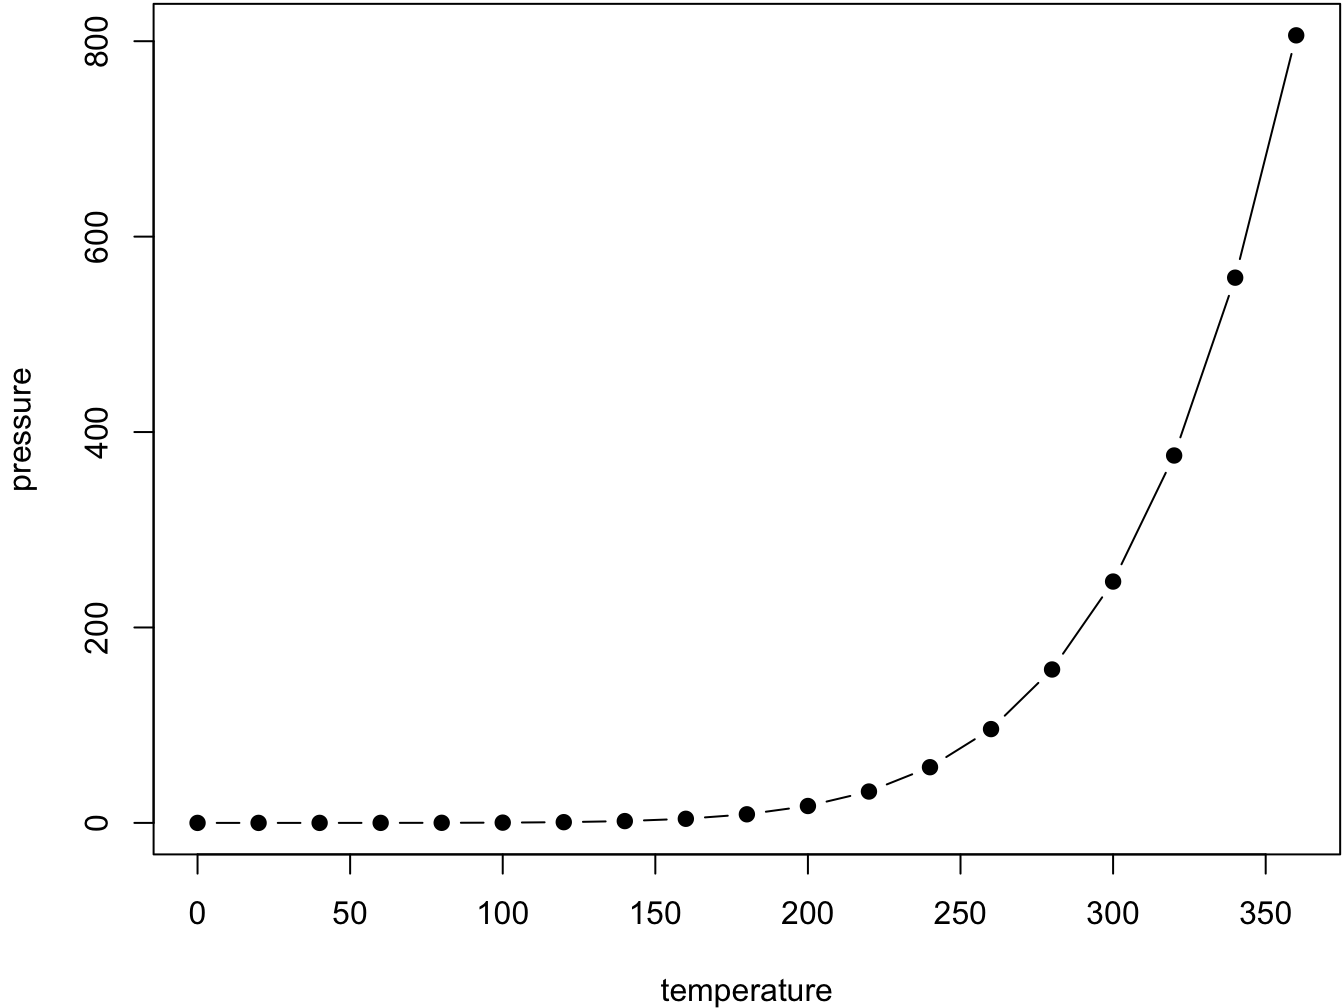
\includegraphics[width=0.65\linewidth]{./_main_files/figure-html/nice-fig-1} \end{center}

\begin{quote}
Ph.D.~student, Courtot Lab
University of Toronto \textbar{} Ontario Institute for Cancer Research
Toronto, ON, Canada

--- \href{mailto:amelanidelahoz@oicr.on.ca}{\nolinkurl{amelanidelahoz@oicr.on.ca}}
\end{quote}

Andres is a Software Engineer with a MSc in Business Information Technologies, who is
currently pursuing his PhD in Medical Biophysics at the University of Toronto. Previously,
Andres was a professor and project coordinator for programming courses at Universidad de
Los Andes, Colombia. His main interests are Artificial Intelligence, software development, and
data analytics. Currently, his PhD project applies AI, specifically Natural Language
Processing, Large Language Models and Knowledge Representation and Reasoning, to
healthcare scenarios.

\subsection*{\texorpdfstring{Amin Noorani (he/him) }{Amin Noorani  (he/him) }}\label{amin-noorani-hehim}
\addcontentsline{toc}{subsection}{Amin Noorani (he/him) }

\begin{center}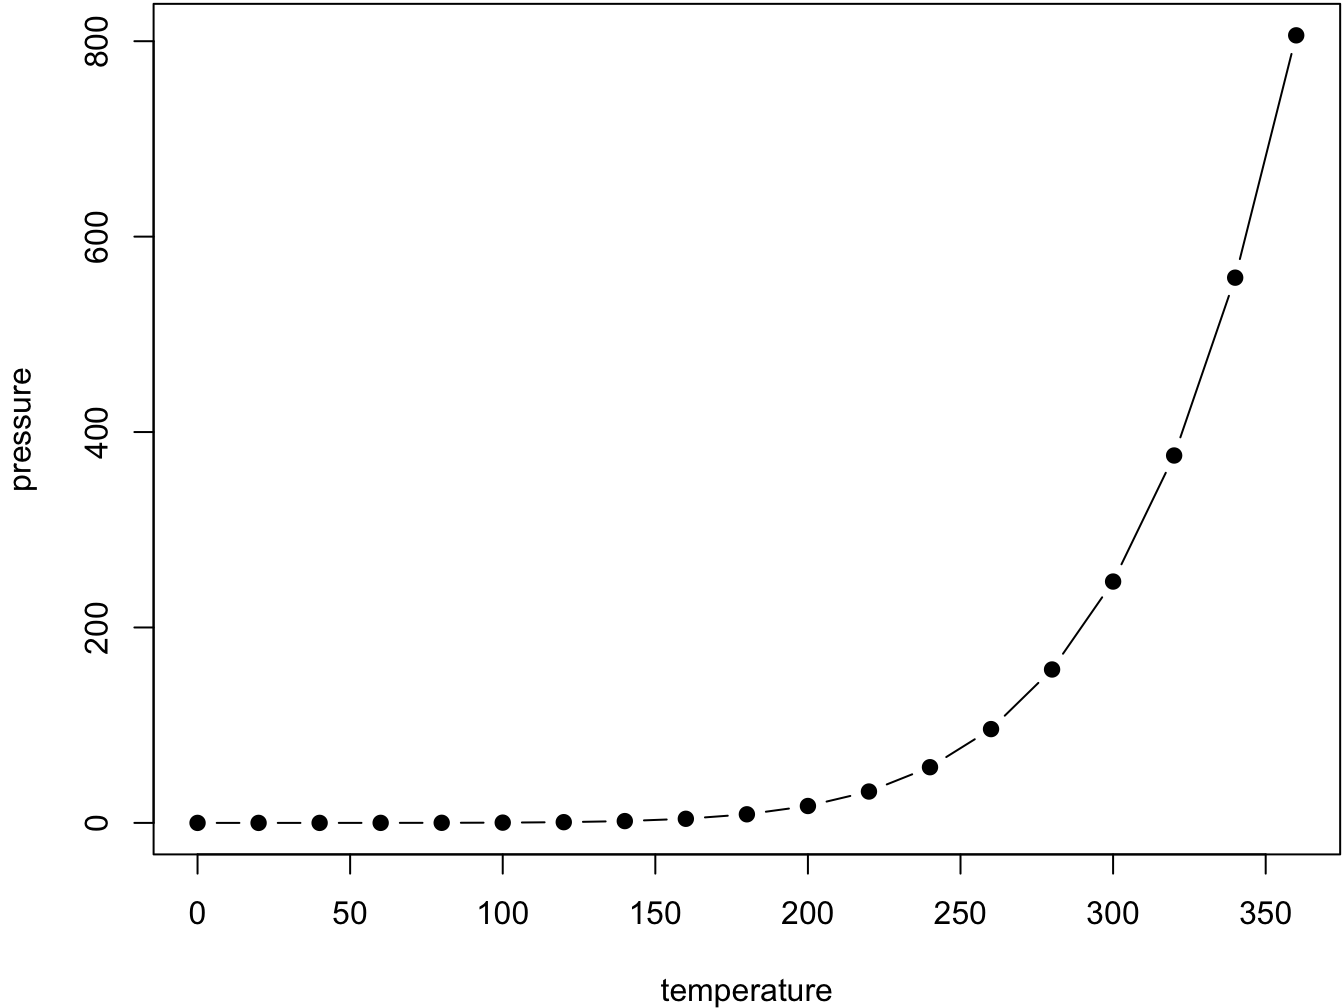
\includegraphics[width=0.65\linewidth]{./_main_files/figure-html/nice-fig-1} \end{center}

\begin{quote}
Master Student \textbar{} Bioinformatician
Toronto Metropolitan University (Olson Lab)
Princess Margaret Genomic Centre (Epigenome Lab)
Toronto, ON, Canada

--- \href{mailto:amin.noorani@uhn.ca}{\nolinkurl{amin.noorani@uhn.ca}}
\end{quote}

Amin is a bioinformatician at Princess Margaret Genomic Centre (PMGC) who is also
pursuing his master's degree at Olson Lab at Toronto Metropolitan University (TMU). Prior to
his current roles, he earned his bachelor's degree in Bioinformatics and started his current
position at PMGC in 2022. His expertise includes analyzing various types of data, including
epigenomics and genomics, from raw data to visualization. His master's project focuses on
exploring gene expression data in ovarian cancer cell lines, as well as image classification to
determine whether cell images have been treated with various compounds.

\subsection*{\texorpdfstring{Zoe Klein (she/her) }{Zoe Klein  (she/her) }}\label{zoe-klein-sheher}
\addcontentsline{toc}{subsection}{Zoe Klein (she/her) }

\begin{center}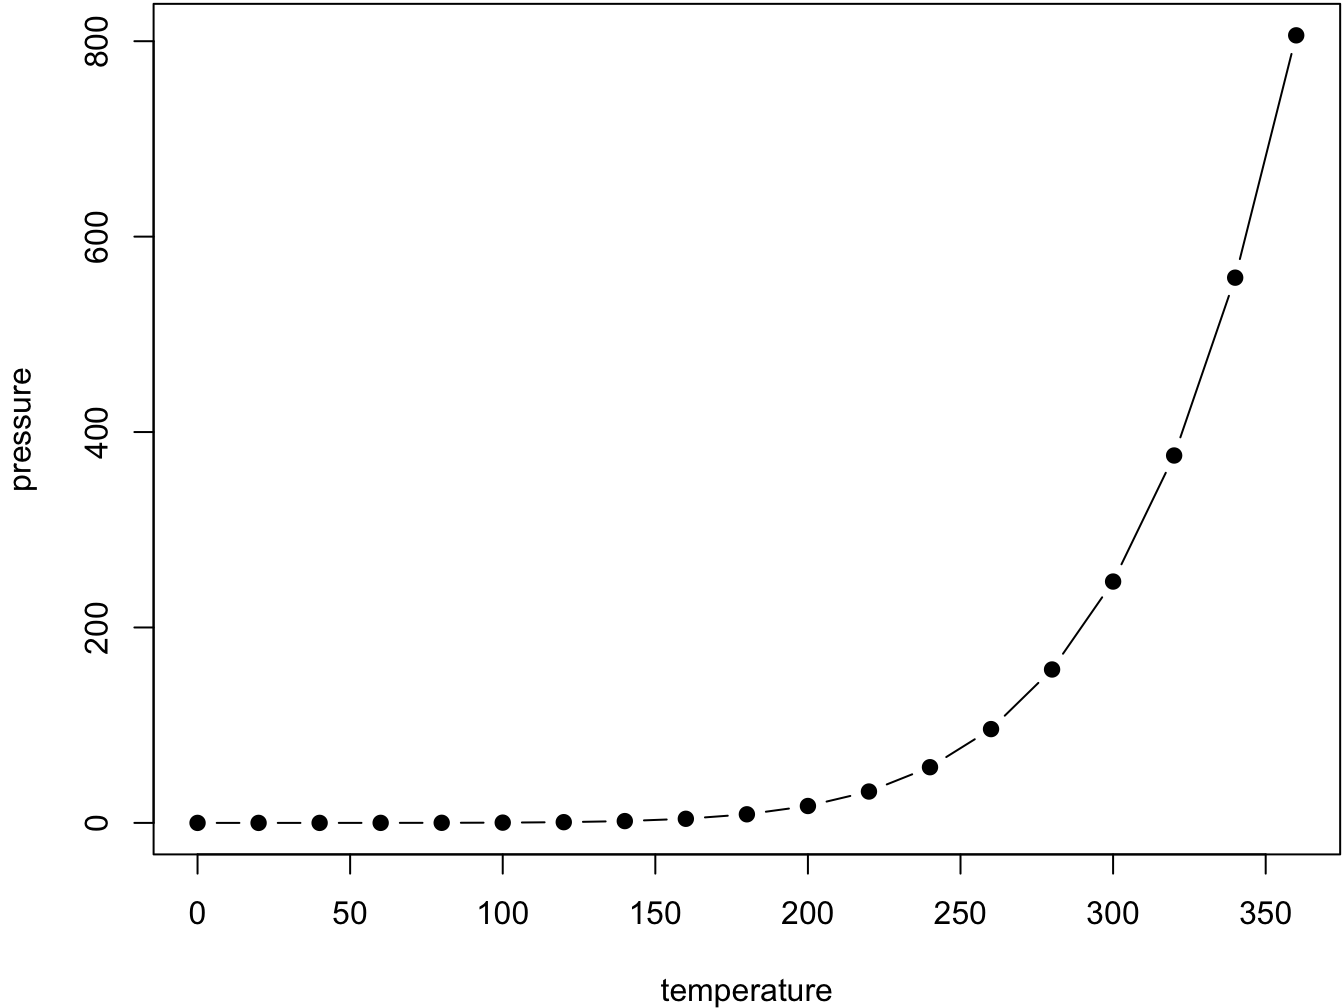
\includegraphics[width=0.65\linewidth]{./_main_files/figure-html/nice-fig-1} \end{center}

\begin{quote}
PhD Candidate, Reimand Lab
University of Toronto

--- \href{mailto:z.klein@mail.utoronto.ca}{\nolinkurl{z.klein@mail.utoronto.ca}}
\end{quote}

Zoe Klein is a PhD candidate at the University of Toronto and the Ontario Institute for Cancer
Research. She uses large-scale data analytics and machine learning to study the role of
non-coding RNA transcripts in cancer.

\subsection*{\texorpdfstring{Michelle Brazas, PhD (she/her) }{Michelle Brazas, PhD  (she/her) }}\label{michelle-brazas-phd-sheher}
\addcontentsline{toc}{subsection}{Michelle Brazas, PhD (she/her) }

\begin{center}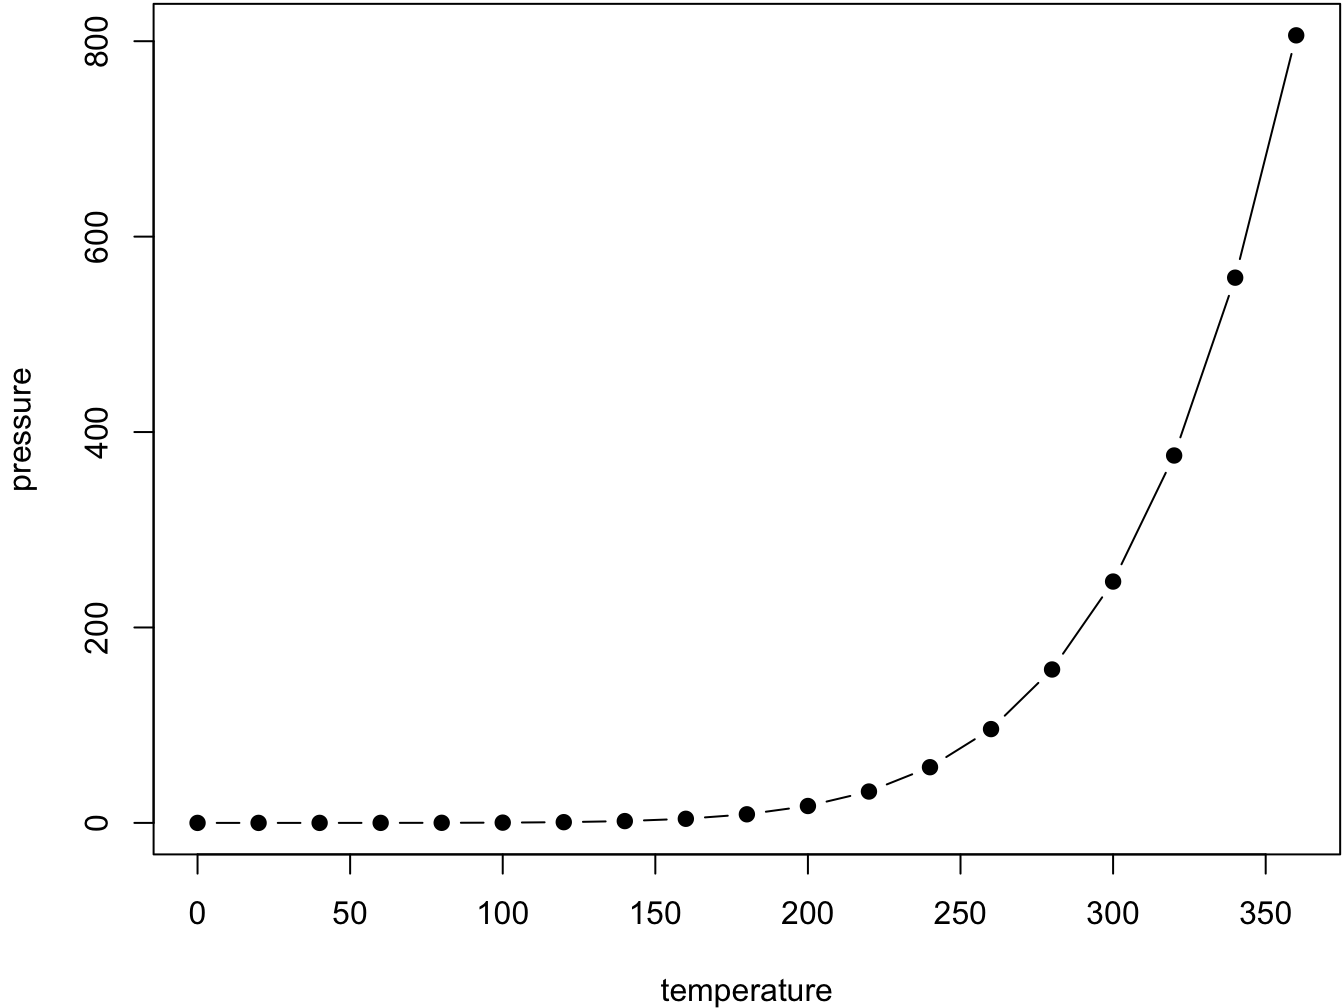
\includegraphics[width=0.65\linewidth]{./_main_files/figure-html/nice-fig-1} \end{center}

\begin{quote}
Scientific Director
Canadian Bioinformatics Workshops (CBW)
Toronto, ON, CA

--- \href{mailto:support@bioinformatics.ca}{\nolinkurl{support@bioinformatics.ca}}
\end{quote}

Dr.~Michelle Brazas is the Associate Director for Adaptive Oncology at the Ontario Institute for
Cancer Research (OICR), and acting Scientific Director at Bioinformatics.ca. Previously, Dr.
Brazas was the Program Manager for Bioinformatics.ca and a faculty member in
Biotechnology at BCIT. Michelle co-founded and runs the Toronto Bioinformatics User Group
(TorBUG) now in its 11th season, and plays an active role in the International Society of
Computational Biology where she sits on the Board of Directors and Executive Board.

\subsection*{\texorpdfstring{Nia Hughes (she/her) }{Nia Hughes  (she/her) }}\label{nia-hughes-sheher}
\addcontentsline{toc}{subsection}{Nia Hughes (she/her) }

\begin{center}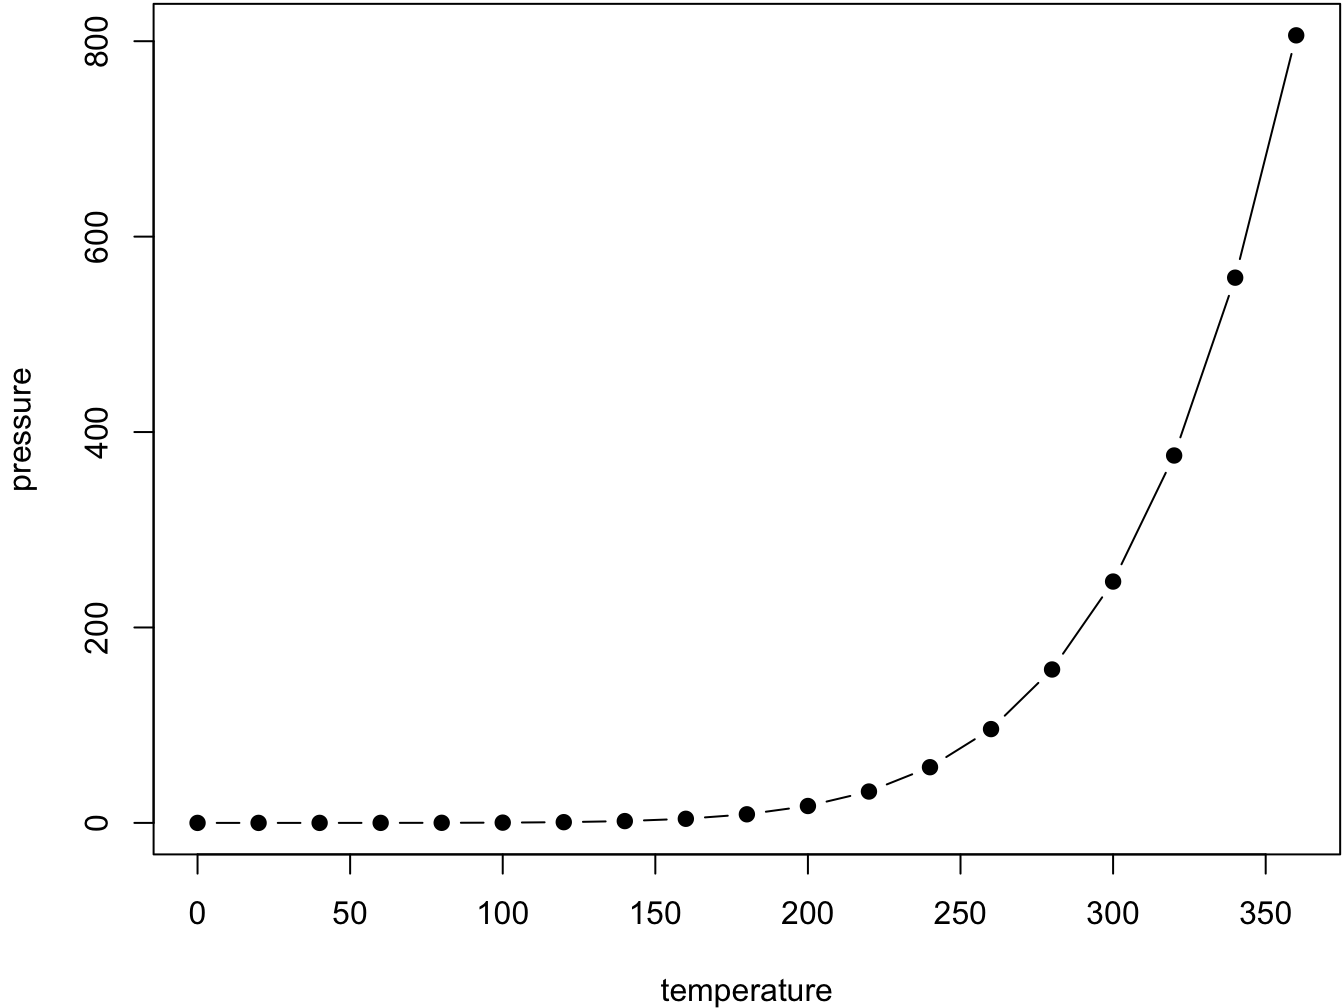
\includegraphics[width=0.65\linewidth]{./_main_files/figure-html/nice-fig-1} \end{center}

\begin{quote}
Program Manager, Bioinformatics.ca
Ontario Institute for Cancer Research
Toronto, ON, Canada

--- \href{mailto:nia.hughes@oicr.on.ca}{\nolinkurl{nia.hughes@oicr.on.ca}}
\end{quote}

Nia is the Program Manager for Bioinformatics.ca, where she coordinates the Canadian
Bioinformatics Workshop Series. Prior to starting at OICR, she completed her M.Sc. in
Bioinformatics from the University of Guelph in 2020 before working there as a
bioinformatician studying epigenetic and transcriptomic patterns across maize varieties.

\chapter{Course Schedule}\label{course-schedule}

\begin{longtable}[]{@{}
  >{\centering\arraybackslash}p{(\columnwidth - 8\tabcolsep) * \real{0.2679}}
  >{\centering\arraybackslash}p{(\columnwidth - 8\tabcolsep) * \real{0.3155}}
  >{\centering\arraybackslash}p{(\columnwidth - 8\tabcolsep) * \real{0.0714}}
  >{\centering\arraybackslash}p{(\columnwidth - 8\tabcolsep) * \real{0.3274}}
  >{\raggedright\arraybackslash}p{(\columnwidth - 8\tabcolsep) * \real{0.0179}}@{}}
\toprule\noalign{}
\begin{minipage}[b]{\linewidth}\centering
CBW's Introduction to R workshop (INR) 2024
\end{minipage} & \begin{minipage}[b]{\linewidth}\centering
\end{minipage} & \begin{minipage}[b]{\linewidth}\centering
\end{minipage} & \begin{minipage}[b]{\linewidth}\centering
\end{minipage} & \begin{minipage}[b]{\linewidth}\raggedright
\end{minipage} \\
\midrule\noalign{}
\endhead
\bottomrule\noalign{}
\endlastfoot
Day 1 & & Day 2 & & \\
June 11 & & June 12 & & \\
Time (EDT) & Module & Time (EDT) & Module & \\
8:30 & Arrivals \& Check-in & 8:30 & Arrivals & \\
9:00 & Welcome (Nia Hughes) & 9:00 & Review \& Module 3: Loops and functions (Frances Wong) & \\
9:30 & Module 1: Getting to Know R (Frances Wong) & 10:00 & Break (15min) & \\
10:30 & Break (15min) & 10:15 & Module 3: Loops and functions (cont'd) & \\
10:45 & Module 1: Getting to Know R (cont'd) & 11:00 & Break (15min) & \\
11:15 & Break (15min) & 11:15 & Module 3: Loops and functions (cont'd) & \\
11:30 & Module 1: Getting to Know R (cont'd) & 12:00 & Class Photo + Break (1h) & \\
12:00 & Break (1h) & 13:00 & Module 4: Linear regression (Frances Wong) & \\
13:00 & Module 2: Exploring your data in R (Frances Wong) & 14:00 & Break (15min) & \\
14:00 & Break (15min) & 14:15 & Module 4: Linear regression (cont'd) & \\
14:15 & Module 2: Exploring your data in R (cont'd) & 15:15 & Break (15min) & \\
15:15 & Break (15min) & 15:30 & Short Project & \\
15:30 & Review and Short project & 17:00 & Survey \& Closing Remarks & \\
17:30 & Finished & 17:30 & Finished & \\
\end{longtable}

\chapter{Cross-references}\label{cross}

calendar(cal\_demo\_data(``week''), view = ``week'', defaultDate = Sys.Date()) \%\textgreater\%
cal\_week\_options(
startDayOfWeek = 1,
workweek = TRUE
) \%\textgreater\%
cal\_props(cal\_demo\_props())

\chapter{Parts}\label{parts}

You can add parts to organize one or more book chapters together. Parts can be inserted at the top of an .Rmd file, before the first-level chapter heading in that same file.

Add a numbered part: \texttt{\#\ (PART)\ Act\ one\ \{-\}} (followed by \texttt{\#\ A\ chapter})

Add an unnumbered part: \texttt{\#\ (PART\textbackslash{}*)\ Act\ one\ \{-\}} (followed by \texttt{\#\ A\ chapter})

Add an appendix as a special kind of un-numbered part: \texttt{\#\ (APPENDIX)\ Other\ stuff\ \{-\}} (followed by \texttt{\#\ A\ chapter}). Chapters in an appendix are prepended with letters instead of numbers.

\chapter{Footnotes and citations}\label{footnotes-and-citations}

\section{Footnotes}\label{footnotes}

Footnotes are put inside the square brackets after a caret \texttt{\^{}{[}{]}}. Like this one \footnote{This is a footnote.}.

\section{Citations}\label{citations}

Reference items in your bibliography file(s) using \texttt{@key}.

For example, we are using the \textbf{bookdown} package \citep{R-bookdown} (check out the last code chunk in index.Rmd to see how this citation key was added) in this sample book, which was built on top of R Markdown and \textbf{knitr} \citep{xie2015} (this citation was added manually in an external file book.bib).
Note that the \texttt{.bib} files need to be listed in the index.Rmd with the YAML \texttt{bibliography} key.

The RStudio Visual Markdown Editor can also make it easier to insert citations: \url{https://rstudio.github.io/visual-markdown-editing/\#/citations}

\chapter{Blocks}\label{blocks}

\section{Equations}\label{equations}

Here is an equation.

\begin{equation} 
  f\left(k\right) = \binom{n}{k} p^k\left(1-p\right)^{n-k}
  \label{eq:binom}
\end{equation}

You may refer to using \texttt{\textbackslash{}@ref(eq:binom)}, like see Equation \eqref{eq:binom}.

\section{Theorems and proofs}\label{theorems-and-proofs}

Labeled theorems can be referenced in text using \texttt{\textbackslash{}@ref(thm:tri)}, for example, check out this smart theorem \ref{thm:tri}.

\begin{theorem}
\protect\hypertarget{thm:tri}{}\label{thm:tri}For a right triangle, if \(c\) denotes the \emph{length} of the hypotenuse
and \(a\) and \(b\) denote the lengths of the \textbf{other} two sides, we have
\[a^2 + b^2 = c^2\]
\end{theorem}

Read more here \url{https://bookdown.org/yihui/bookdown/markdown-extensions-by-bookdown.html}.

\section{Callout blocks}\label{callout-blocks}

The R Markdown Cookbook provides more help on how to use custom blocks to design your own callouts: \url{https://bookdown.org/yihui/rmarkdown-cookbook/custom-blocks.html}

\chapter{Sharing your book}\label{sharing-your-book}

\section{Publishing}\label{publishing}

HTML books can be published online, see: \url{https://bookdown.org/yihui/bookdown/publishing.html}

\section{404 pages}\label{pages}

By default, users will be directed to a 404 page if they try to access a webpage that cannot be found. If you'd like to customize your 404 page instead of using the default, you may add either a \texttt{\_404.Rmd} or \texttt{\_404.md} file to your project root and use code and/or Markdown syntax.

\section{Metadata for sharing}\label{metadata-for-sharing}

Bookdown HTML books will provide HTML metadata for social sharing on platforms like Twitter, Facebook, and LinkedIn, using information you provide in the \texttt{index.Rmd} YAML. To setup, set the \texttt{url} for your book and the path to your \texttt{cover-image} file. Your book's \texttt{title} and \texttt{description} are also used.

This \texttt{gitbook} uses the same social sharing data across all chapters in your book- all links shared will look the same.

Specify your book's source repository on GitHub using the \texttt{edit} key under the configuration options in the \texttt{\_output.yml} file, which allows users to suggest an edit by linking to a chapter's source file.

Read more about the features of this output format here:

\url{https://pkgs.rstudio.com/bookdown/reference/gitbook.html}

Or use:

\begin{Shaded}
\begin{Highlighting}[]
\NormalTok{?bookdown}\SpecialCharTok{::}\NormalTok{gitbook}
\end{Highlighting}
\end{Shaded}

\chapter{R Markdown}\label{r-markdown}

point

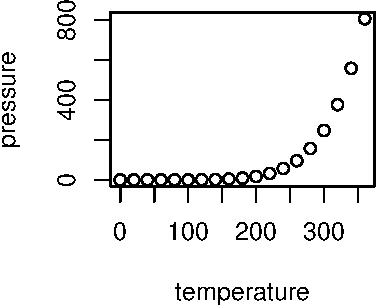
\includegraphics{_main_files/figure-latex/pressure-plot-1.pdf}

This is an R Markdown document. Markdown is a simple formatting syntax for authoring HTML, PDF, and MS Word documents. For more details on using R Markdown see \url{http://rmarkdown.rstudio.com}.

When you click the \textbf{Knit} button a document will be generated that includes both content as well as the output of any embedded R code chunks within the document. You can embed an R code chunk like this:

Note that the \texttt{echo\ =\ FALSE} parameter was added to the code chunk to prevent printing of the R code that generated the plot.

\begin{Shaded}
\begin{Highlighting}[]
\FunctionTok{cat}\NormalTok{(}\StringTok{"just as it *is*"}\NormalTok{)}
\end{Highlighting}
\end{Shaded}

just as it \emph{is}

\begin{Shaded}
\begin{Highlighting}[]
\FunctionTok{library}\NormalTok{(knitr)}
\FunctionTok{kable}\NormalTok{(cars)}
\end{Highlighting}
\end{Shaded}

\begin{tabular}{r|r}
\hline
speed & dist\\
\hline
4 & 2\\
\hline
4 & 10\\
\hline
7 & 4\\
\hline
7 & 22\\
\hline
8 & 16\\
\hline
9 & 10\\
\hline
10 & 18\\
\hline
10 & 26\\
\hline
10 & 34\\
\hline
11 & 17\\
\hline
11 & 28\\
\hline
12 & 14\\
\hline
12 & 20\\
\hline
12 & 24\\
\hline
12 & 28\\
\hline
13 & 26\\
\hline
13 & 34\\
\hline
13 & 34\\
\hline
13 & 46\\
\hline
14 & 26\\
\hline
14 & 36\\
\hline
14 & 60\\
\hline
14 & 80\\
\hline
15 & 20\\
\hline
15 & 26\\
\hline
15 & 54\\
\hline
16 & 32\\
\hline
16 & 40\\
\hline
17 & 32\\
\hline
17 & 40\\
\hline
17 & 50\\
\hline
18 & 42\\
\hline
18 & 56\\
\hline
18 & 76\\
\hline
18 & 84\\
\hline
19 & 36\\
\hline
19 & 46\\
\hline
19 & 68\\
\hline
20 & 32\\
\hline
20 & 48\\
\hline
20 & 52\\
\hline
20 & 56\\
\hline
20 & 64\\
\hline
22 & 66\\
\hline
23 & 54\\
\hline
24 & 70\\
\hline
24 & 92\\
\hline
24 & 93\\
\hline
24 & 120\\
\hline
25 & 85\\
\hline
\end{tabular}

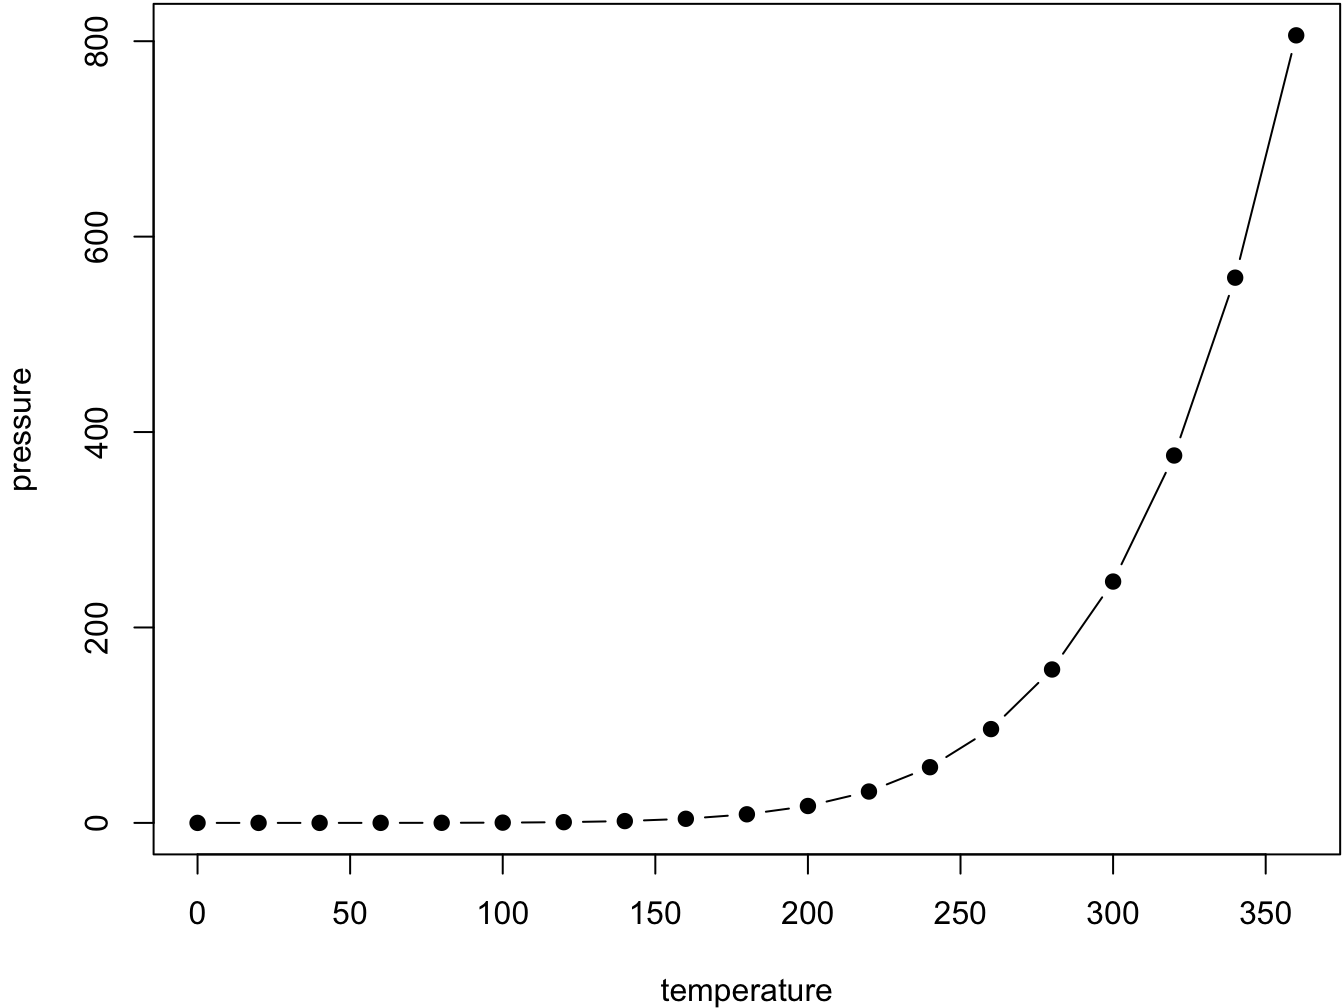
\includegraphics{./_main_files/figure-html/nice-fig-1.png}

  \bibliography{book.bib,packages.bib}

\end{document}
